\newpage\ \newpage\section{Introduction} Isaac Asimov, the prolific American author, once wrote that \begin{quote} The most exciting phrase to hear [...], the one that heralds the most discoveries, is not ``Eureka!'' but ``That's funny...''.\end{quote}
However, anomalous observations are not only harbingers of great scientific discoveries -- unexpected observations can spoil analyses or be indicative of the presence of issues related to data collection or data processing. \par Either way, it becomes imperative for decision-makers and analysts to establish anomaly detection protocols, and to identify strategies to deal with such observations.  
\subsection{Basic Notions and Overview}
\textbf{Outlying observations} are data points which are \textbf{atypical} in comparison to the unit's remaining features (\textit{within-unit}), or in comparison to the measurements for other units (\textit{between-units}), or as part of a collective subset of observations. Outliers are thus observations which are \textbf{dissimilar to other cases} or which contradict \textbf{known dependencies} or rules.\footnote{Outlying observations may be anomalous along any of the individual variables, or in combination.}% (information in this section is taken partly from \cite{DP_OW,DP_A,DP_T,DP_CBK}).
\par Observations could be anomalous in one context, but not in another. Consider, for instance, an adult male who is 6-foot tall. Such a man would fall in the 86th percentile among Canadian males \cite{DP_HPC}, which, while on the tall side, is not unusual; in Bolivia, however, the same man would land in the 99.9th percentile \cite{DP_HPC}, which would mark him as extremely tall and quite dissimilar to the rest of the population.\footnote{Anomaly detection points towards interesting questions for analysts and subject matter experts: in this case, why is there such a large discrepancy in the two populations?}  
\newl
A common mistake that analysts make when dealing with outlying observations is to remove them from the dataset without carefully studying whether they are \textbf{influential data points}, that is, observations whose absence leads to \textbf{markedly different} analysis results.\par When influential observations are identified, remedial measures (such as data transformation strategies) may need to be applied to minimize any undue effect. Note that outliers may be influential, and influential data points may be outliers, but the conditions are neither necessary nor sufficient. 
\newl
Numerous methods exist to identify anomalous observations; \textbf{none of them are foolproof} and judgement must be used. Methods that employ graphical aids (such as box-plots, scatterplots, scatterplot matrices, and 2D tours) to identify outliers are particularly easy to implement, but a low-dimensional setting is usually required for ease of interpretability. \par Analytical methods also exist (using Cooke's or Mahalanobis' distances, say), but in general some additional level of analysis must be performed, especially when trying to identify influential points (\textit{cf.} \textbf{leverage}). 
\newl With small datasets, anomaly detection can be conducted on a case-by-case basis, but with large datasets, the temptation to use \textbf{automated detection/removal} is strong -- care must be exercised before the analyst decides to go down that route.\footnote{This stems partly from the fact that that once the ``anomalous'' observations have been removed from the data set, previously ``regular'' observations can become anomalous in turn in the smaller dataset; it is not clear when that runaway train will stop.}\par
In the early stages of anomaly detection, \textbf{simple data analyses} (such as descriptive statistics, 1- and 2-way tables, and  traditional visualisations) may be performed to help identify anomalous observations, or to obtain insights about the data, which could eventually lead to modifications of the analysis plan.
\subsubsection*{Outlier Tests} How are outliers \textit{actually} detected? Most methods come in one of two flavours: \textbf{supervised} and \textbf{unsupervised} (we will discuss those in detail in later sections).\par
Supervised methods use a historical record of \textbf{labeled} (that is to say, previously identified) anomalous observations to build a \textbf{predictive classification or regression model} which estimates the probability that a unit is anomalous; domain expertise is required to tag the data. Since anomalies are typically \textbf{infrequent}, these models often also have to accommodate the \textbf{rare occurrence problem}.\footnote{Supervised models are built to minimize a cost function; in default settings, it is often the case that the mis-classification cost is assumed to be symmetrical, which can lead to technically correct but useless solutions. For instance, the vast majority (99.999+\%) of air passengers emphatically do not bring weapons with them on flights; a model that predicts that no passenger is attempting to smuggle a weapon on board a flight would be 99.999+\% accurate, but it would miss the point completely.}\par Unsupervised methods, on the other hand, use no previously labeled information or data, and try to determine if an observation is an outlying one solely by comparing its behaviour to that of the other observations. \newpage\noindent The following traditional methods and tests of outlier detection fall into this category:\footnote{Note that \textbf{normality} of the underlying data is an assumption for most tests; how robust these tests are against departures from this assumption depends on the situation.}
\begin{itemize}[noitemsep]
\item Perhaps the most commonly-used test is \textbf{Tukey's boxplot test}; for normally distributed data, regular observations typically lie between the \textbf{inner fences} $$Q_1-1.5(Q_3-Q_1) \quad\mbox{and}\quad Q_3+1.5(Q_3-Q_1).$$ \textbf{Suspected outliers} lie between the inner fences and the \textbf{outer fences} 
$$Q_1-3(Q_3-Q_1) \quad\mbox{and}\quad Q_3+3(Q_3-Q_1).$$
Points beyond the outer fences are identified as \textbf{outliers} ($Q_1$ and $Q_3$ represent the data's   $1^{\textrm{st}}$ and $3^{\textrm{rd}}$ quartile, respectively; see Figure~\ref{fig:boxplot}).
\begin{figure}[t]
\centering
\includegraphics[width=0.30\textwidth]{Images/boxplot_\ldoc.png}
\caption[\small Tukey's boxplot test for outliers]{\small Tukey's boxplot test; suspected outliers are marked by white disks, outliers by black disks.}
\hrule\label{fig:boxplot}
\end{figure}
\afterpage{\FloatBarrier}
\item The \textbf{Grubbs test} is another univariate test, which takes into consideration the number of observations in the dataset. Let $x_i$ be the value of feature $X$ for the $i^{\textrm{th}}$ unit, $1\leq i\leq N$, let $(\overline{x},s_x)$ be the mean and standard deviation of feature $X$, let $\alpha$ be the desired significance level, and let  $T(\alpha,N)$ be the critical value of the Student $t$-distribution at significance $\alpha/2N$. Then, the $i^{\textrm{th}}$ unit is an \textbf{outlier along feature} $X$ if $$|x_i-\overline{x}| \geq \frac{s_x(N-1)}{\sqrt{N}}\sqrt{\frac{T^2(\alpha,N)}{N-2+T^2(\alpha,N)}}.$$
\item Other common tests include:
\begin{itemize}[noitemsep]
\item the \textbf{Dixon $Q$ test}, which is used in the experimental sciences to find outliers in (extremely) small datasets -- it is of dubious validity;
\item the \textbf{Mahalanobis distance}, which is linked to the leverage of an observation (a measure of influence), can also be used to find multi-dimen\-sio\-nal outliers, when all relationships are linear (or nearly linear);
\item the \textbf{Tietjen-Moore} test, which is used to find a specific number of outliers;
\item the \textbf{generalized extreme studentized deviate} test, if the number of outliers is unknown; 
\item the \textbf{chi-square} test, when outliers affect the goodness-of-fit, as well as 
\item DBSCAN and other clustering-based outlier detection methods.
\end{itemize}
\end{itemize}
\subsubsection*{Visual Outlier Detection} The following three (simple) examples illustrate the principles underlying visual outlier and anomaly detection. 
\begin{Example}On a specific day, the height of several plants in a nursery are measured. The records also show each plant's age (the number of weeks since the seed has been planted). 
\begin{figure*}[t]
\centering
\includegraphics[width=0.32\textwidth]{Images/plant_age_\ldoc}\quad
\includegraphics[width=0.32\textwidth]{Images/plant_height_\ldoc}\quad
\includegraphics[width=0.32\textwidth]{Images/plant_height_vs_age_\ldoc}
\caption[\small Summary visualisations for a plant dataset]{\small Summary visualisations for an (artificial) plant dataset: age distribution (left), height distribution (middle), height vs. age, with linear trend (right).} \label{fig:plant_data}
\end{figure*}
\begin{figure*}[t]
\centering
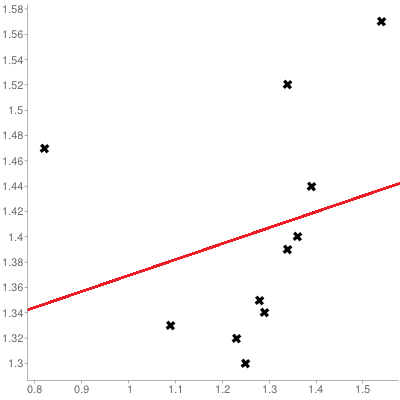
\includegraphics[width=0.32\textwidth]{Images/scatter_plot_linear_1}\quad
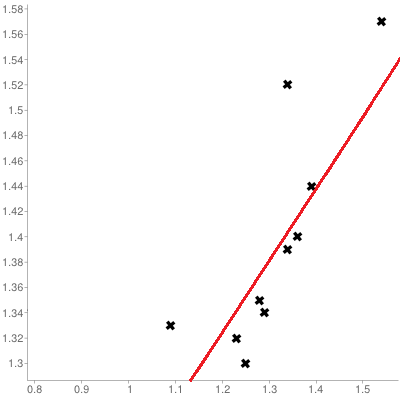
\includegraphics[width=0.32\textwidth]{Images/scatter_plot_linear_2}\quad
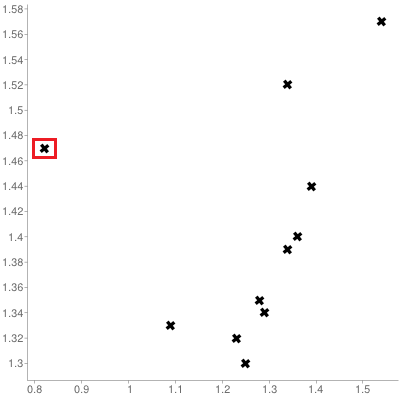
\includegraphics[width=0.32\textwidth]{Images/scatter_plot_2}
\caption[\small Visualisations for a service point dataset]{\small Visualisations for an (artificial) service point dataset: trend for 11 service points (left), trend for 10 service points (middle), influential observations (right).}\hrule
        \label{fig:service_data}
\end{figure*}
\begin{figure*}[t]
\centering\includegraphics[width=0.26\textwidth]{{Images/appendage_length_descriptive_\ldoc}}\quad \includegraphics[width=0.50\textwidth]{{Images/appendage_length_\ldoc}}
\caption[\small Summary and visualisation for an appendage length dataset]{\small Summary and visualisation for an (artificial) appendage length dataset: descriptive statistics (left), appendge length distribution (right).}\hrule
\label{tab:appendage_data}
\end{figure*}

Histograms of the data are shown in Figure~\ref{fig:plant_data} (age on the left, height on the middle). \par Very little can be said about the data at that stage: the age of the plants (controlled by the nursery staff) seems to be somewhat haphazard, as does the response variable (height). A scatter plot of the data (rightmost chart in Figure~\ref{fig:plant_data}), however, reveals that growth is strongly correlated with age during the early period of a plant's life for the observations in the dataset; points clutter around a linear trend. One point (in yellow) is easily identified as an \textbf{outlier}. There are (at least) two possibilities: either that measurement was botched or mis-entered in the database (representing an invalid entry), or that one specimen has experienced unusual growth (outlier). Either way, the analyst has to investigate further.  
  \end{Example}
  \begin{Example}
A government department has 11 service points in a jurisdiction. Service statistics are recorded: the monthly average arrival rates per teller and monthly average service rates per teller for each service point are available. \par A scatter plot of the service rate per teller ($y$ axis) against the arrival rate per teller ($x$ axis), with linear regression trend, is shown in the leftmost chart in Figure~\ref{fig:service_data}. The trend is seen to inch upwards with increasing $x$ values. \par A similar chart, but with the left-most point removed from consideration, is shown in the middle chart of  Figure~\ref{fig:service_data}. The trend still slopes upward, but the fit is significantly improved, suggesting that the removed observation is unduly \textbf{influential} (or anomalous) -- a better understanding of the relationship between arrivals and services is afforded if it is set aside. \par Any attempt to fit that data point into the model must take this information into consideration. Note, however, that influential observations depend on the analysis that is ultimately being conducted -- a point may be influential for one analysis, but not for another.     
\end{Example}
\begin{Example}
Measurements of the length of the appendage of a certain species of insect have been made on 71 individuals. Descriptive statistics have been computed; the results are shown in Figure~\ref{tab:appendage_data}.

\newpage\noindent Analysts who are well-versed in statistical methods might recognize the tell-tale signs that the distribution of appendage lengths is likely to be asymmetrical (since the skewness is non-negligible) and to have a ``fat'' tail (due to the kurtosis being commensurate with the mean and the standard deviation, the range being so much larger than the interquartile range, and the maximum value being so much larger than the third quartile). \par The mode, minimum, and first quartile values belong to individuals without appendages, so there appears to be at least two sub-groups in the population (perhaps split along the lines of juveniles/adults, or males/females). The maximum value has already been seen to be quite large compared to the rest of the observations, which at first suggests that it might belong to an \textbf{outlier}. \par The histogram of the measurements, however, shows that there are 3 individuals with very long appendages (see right-most chart in Figure~\ref{tab:appendage_data}): it now becomes plausible for these anomalous entries to belong to individuals from a different species altogether who were \textbf{erroneously added} to the dataset. This does not, of course, constitute a proof of such an error, but it raises the possibility, which is often the best that an analyst can do in the absence of subject matter expertise.
\end{Example}
\noindent This traditional approach to anomaly detection fails for high-dimensional datasets, however, and a fundamentally different approach is advocated.\newpage  
\subsection{Anomaly Detection as a Statistical Learning Problem}
Fraudulent behaviour is not always easily identifiable, even after the fact. Credit card fraudsters, for instance, will try to disguise their transactions as regular and banal, rather than as outlandish; to fool human observers into confusing what is merely \textbf{plausible} with what is \textbf{probable} (or at least, \textbf{not improbable}).\newl At its most basic level, anomaly detection is a problem in \textbf{applied probability}: if $I$ denotes what is known about the dataset (behaviour of individual observations, behaviour of observations as a group, anomalous/normal verdict for a number of similar observations, etc.), is $$P(\text{obs.\@ is anomalous}|I) > P(\text{obs.\@ is normal}|I)?$$ 
Anomaly detection models usually assume \textbf{stationarity for normal observations}, which is to say, that the underlying mechanism that generates data does not change in a substantial manner over time, or, if it does, that its rate of change or cyclicity is known. \newl For time series data, this means that it may be necessary to first perform trend and seasonality extraction.
\begin{Example} Supply chains play a crucial role in the transportation of goods from one part of the world to another. As the saying goes, ``a given chain is only as strong as its weakest link'' -- in a multi-modal context, comparing the various transportation segments is far from an obvious endeavour: if shipments departing Shanghai in February 2013 took two more days, on average, to arrive in Vancouver than those departing in July 2017, can it be said with any certainty that the shipping process has improved in the intervening years? Are February departures always slower to cross the Pacific Ocean? \par The seasonal variability of performance is relevant to supply chain monitoring; the ability to quantify and account for the severity of its impact on the data is thus of great interest. \par 
One way to tackle this problem is to produce an \textbf{index} to track container transit times. This index should depict the \textbf{reliability} and the \textbf{variability} of transit times but in such a way as to be able to allow for performance comparison between differing time periods.\newl 
To simplify the discussion, assume that the ultimate goal is to compare quarterly and/or monthly performance data, irrespective of the transit season, in order to determine how well the network is performing on the \textit{Shanghai} $\to$ \textit{Port Metro Vancouver/Prince Rupert} $\to$ \textit{Toronto} corridor, say. 
\begin{figure}[H]
\centering
\includegraphics[width=0.5\textwidth]{Images/mmsc_\ldoc.png}
\caption{\small Multi-modal supply chain.} \label{fig:mmsc}
\end{figure}
\noindent The supply chain under investigation has Shanghai as the point of origin of shipments, with Toronto as the final destination; the containers enter the country either through Vancouver or Prince Rupert. Containers leave their point of origin by boat, arrive and dwell in either of the two ports before reaching their final destination by rail. \par 
For each of the three segments (Marine Transit, Port Dwell, Rail Transit), the data consists of the monthly empirical distribution of transit times, built from sub-samples  (assumed to be randomly selected and fully representative) of all containers entering the appropriate segment.
\newl
Each segment's performance is measured using \textbf{fluidity indicators}, which are computed using various statistics of the transit/dwelling time distributions for each of the supply chain segments, such as: 
\begin{description}[noitemsep]
\item[Reliability Indicator (RI)] -- the ratio of the 95$^{\text{th}}$ percentile to the 5$^{\text{th}}$ percentile of transit/dwelling times (a high RI indicates high volatility, whereas a low RI $(\approx 1)$ indicates a reliable corridor);
\item[Buffer Index (BI)] -- the ratio of the positive difference between the 95$^{\text{th}}$ percentile and the mean, to the mean. A small BI $(\approx 0)$ indicates only slight variability in the upper (longer) transit/dwelling times; a large BI indicates that the variability of the longer transit/dwelling times is high, and that outliers might be found in that domain;
\item[Coefficient of Variation (CV)] -- the ratio of the standard deviation of transit/dwelling times to the mean transit/dwelling time.  
\end{description}
The time series of monthly indicators (which are derived from the monthly transit/dwelling time distributions in each segment) are then \textbf{decomposed} into their 
\begin{itemize}[noitemsep]
\item trend;
\item seasonal component (seasonality, trading-day, moving-holiday), and 
\item irregular component.
\end{itemize}
\noindent The trend and the seasonal components provide the \textbf{expected behaviour} of the indicator time series;\footnote{Before carrying out seasonal adjustment, it is important to identify and pre-adjust for structural breaks (using the Chow test, for instance), as their presence can give rise to severe distortions in the estimation of the Trend and Seasonal effects. Seasonal breaks occur when the usual seasonal activity level of a particular time reporting unit changes in subsequent years. Trend breaks occurs when the trend in a data series is lowered or raised for a prolonged period, either temporarily or permanently. Sources of these breaks may come from changes in government policies, strike actions, exceptional events, inclement weather, etc.} the irregular component arose as a consequence of supply chain \textbf{volatility}. A high irregular component at a given time point indicates a poor performance against expectations for that month, which is to say, an \textbf{anomalous observation}.  
\begin{figure}[t]
\centering
\includegraphics[width=0.5\textwidth]{Images/decomposition_\ldoc.png}
\caption{\small Conceptual time series decomposition; potential anomalous behaviour should be searched for in the irregular component.}\hrule \label{fig:description}
\end{figure}
\newl In general, the decomposition follows a model which is 
\begin{itemize}[noitemsep]
\item multiplicative;
\item additive, or 
\item pseudo-additive.
\end{itemize}
The choice of a model is driven by data behaviour and choice of assumptions; the X12 model automates some of the aspects of the decomposition, but manual intervention and diagnostics are still required.\footnote{X12 is implemented in SAS and R, among other platforms.}
The additive model, for instance, assumes that: 
\begin{enumerate}[noitemsep]\item the seasonal component $S_t$ and the irregular component $I_t$ are independent of the trend $T_t$; \item  the seasonal component $S_t$ remains stable from year to year; and \item there is no seasonal fluctuation: $\sum_{j=1}^{12} S_{t+j}=0 $.\end{enumerate} 
Mathematically, the model is expressed as:
    \begin{equation*}
        O_t = T_t + S_t + I_t
    \end{equation*}
    All components share the same dimensions and units. After seasonality adjustment,the seasonality adjusted series is:
    \begin{equation*}
        SA_t = O_t - S_t = T_t + I_t
    \end{equation*}
The multiplicative and pseudo-additive models are defined in similar ways (consult \cite{TS_FH,TS_FMBOC,TS_ICTSA,TS_SAETS,TS_JL} for details).\footnote{The simplest way to determine whether to use multiplicative or additive decomposition is by graphing the time series. If the size of the seasonal variation increases/decreases over time, multiplicative decomposition should be used. On the other hand, if the seasonal variation seems to be constant over time, additive model should be used. A pseudo-additive model should be used when the data exhibits the characteristics of the multiplicative series, but parameter values are close to zero.}\newl 
The data decomposition/preparation process is illustrated with the 40-month time series of marine transit CVs from 2010-2013, whose values are shown in Figure~\ref{fig:cv_cont}.  The size of the peaks and troughs seems fairly constant with respect to the changing trend; the SAS implementation of X12 agrees with that assessment and suggests the additive decomposition model, with  no need for further data transformations.
\begin{figure*}[t]
\centering
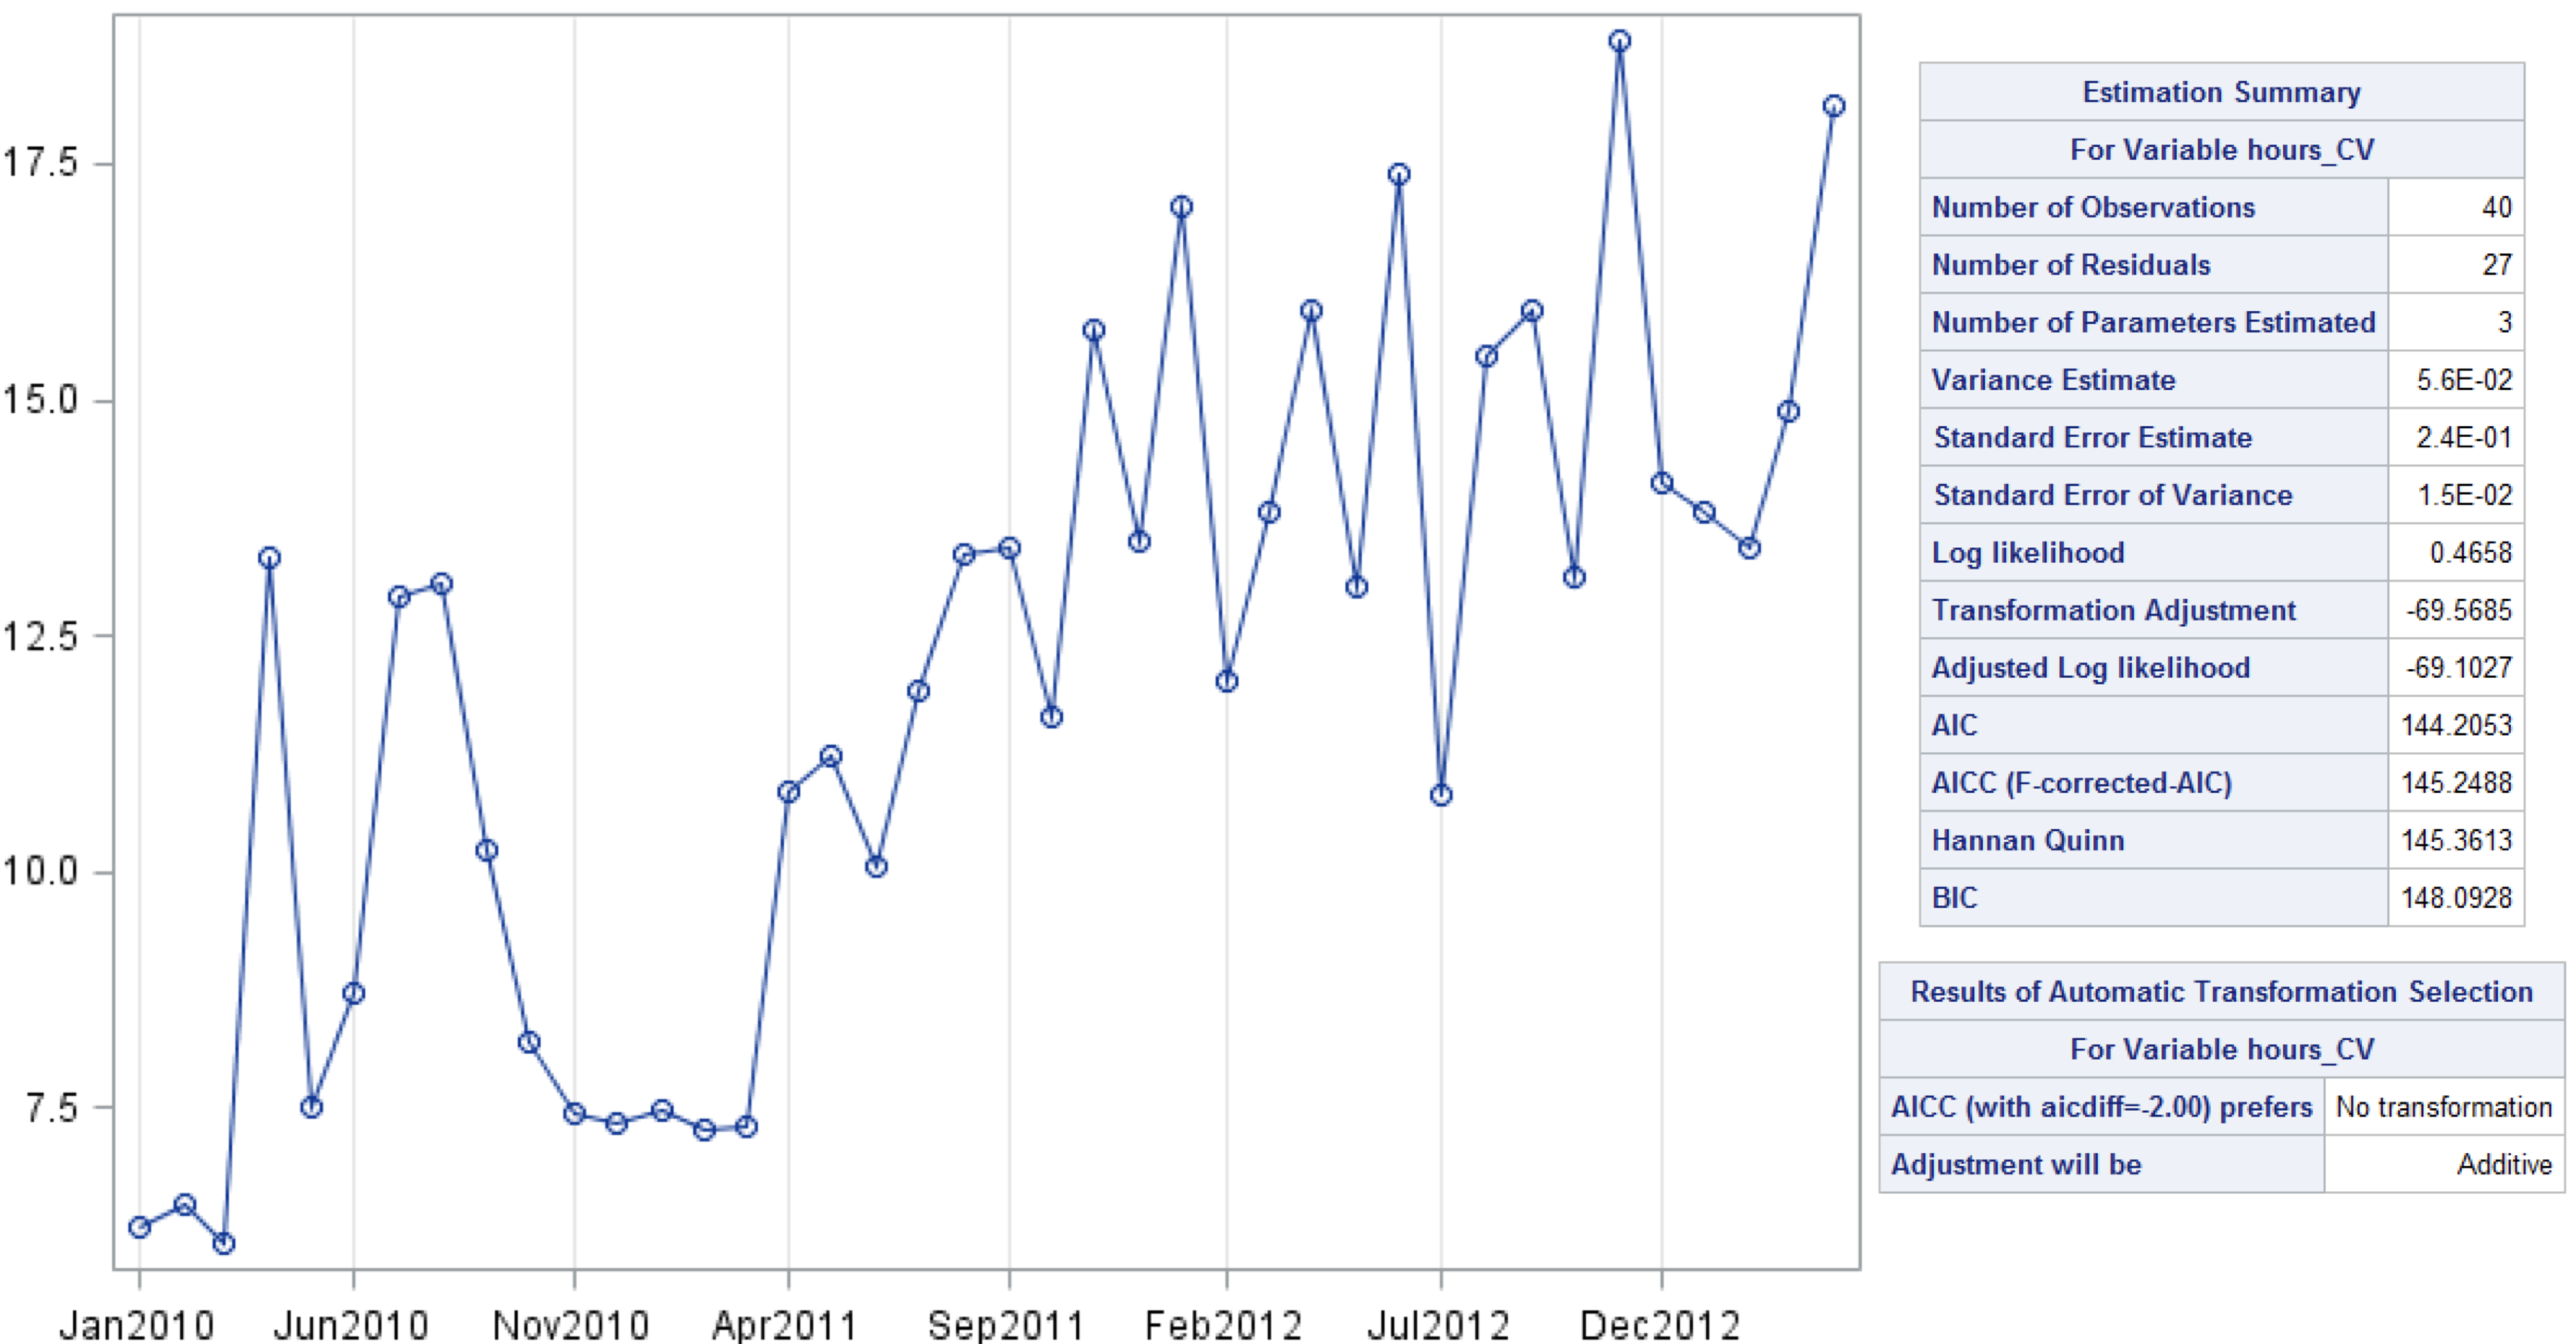
\includegraphics[width=0.75\textwidth]{Images/CV_continuously.png}
\caption{Monthly marine transit CVs and estimation summary.}
\label{fig:cv_cont}
\end{figure*}
\par The diagnostic plots are shown in Figure~\ref{fig:diff}: the CV series is prior-adjusted from the beginning until OCT2010 after the detection of a level shift. The SI (Seasonal Irregular) chart shows that there are more than one irregular component which exhibits volatility.
\begin{figure*}[t]
\centering
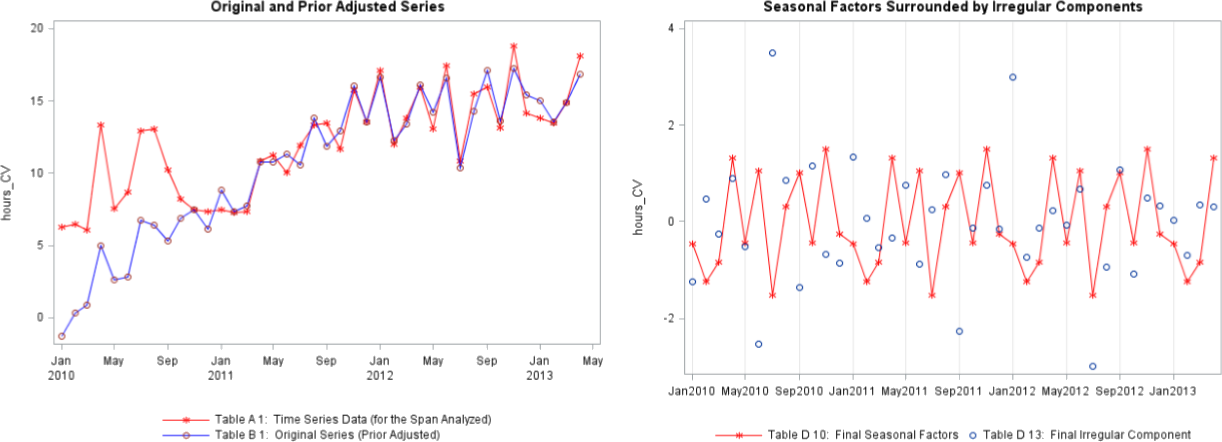
\includegraphics[width=0.98\textwidth]{Images/DiffComponents.png}
\caption[Diagnostic plots.]{Diagnostic plots. Note that the analysis of a time series starts with estimation of the effects of festivals and trading days. These pre-calculated
estimates are then used for prior adjustment of the series. The prior adjusted original series is subsequently analyzed using the seasonal adjustment.}\hrule
\label{fig:diff}
\end{figure*}
The adjusted series is shown below in Figure~\ref{fig:adjusted}; the trend and irregular components are also shown separately for readability. It is on the irregular component that detection anomaly would be conducted. 
\begin{figure*}[t]
\centering
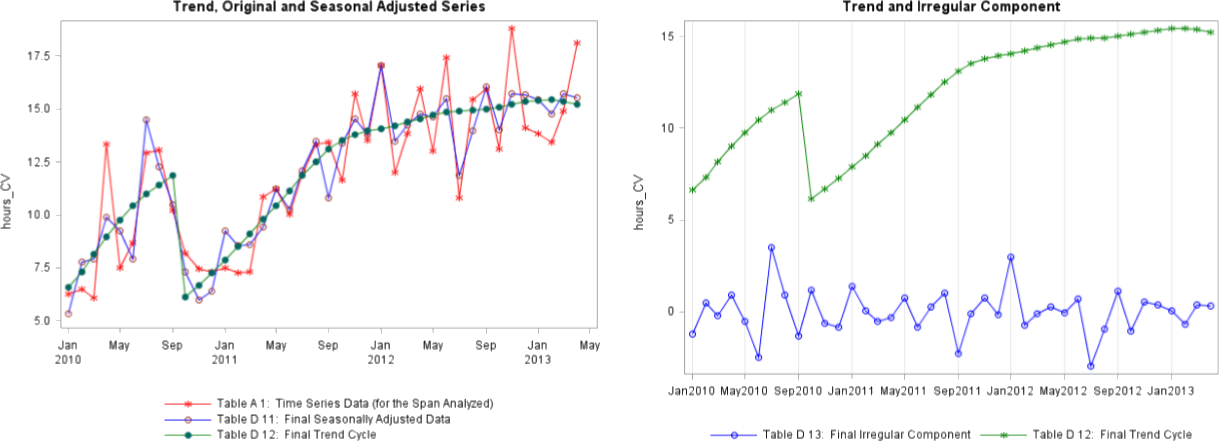
\includegraphics[width=0.98\textwidth]{Images/adjustedplot.png}
\caption{Adjusted time series components plots.}\hrule
\label{fig:adjusted}
\end{figure*}
\end{Example}
\begin{center}
    \rule{0.25\textwidth}{.4pt}
\end{center}
The last example shows the importance of domain understanding and data preparation to the anomaly detection process. Given that the vast majority of observations in a general problem are typically "normal", another conceptually important approach is to view anomaly detection as a \textbf{rare occurrence learning} classification problem or as a \textbf{novelty detection} data stream problem (these problems will be tackled in other data science reports of this series). \par Either way, while there a number of strategies use regular classification/clustering algorithms for anomaly detection, they are rarely successful unless they are adapted or modified for the anomaly detection context.  
\subsubsection*{Basic Concepts}
A generic system (such as the monthly transit times from the previous subsection, say) may be realized in \textbf{normal} states or in \textbf{abnormal} states. Normality, perhaps counter-intuitively, is not confined to finding the most likely state, however, as infrequently occurring states could still be normal or plausible under some interpretation of the system. \par As the authors of \cite{A10} see it, a system's states are the results of processes or behaviours that follow certain natural rules and broad principles; the observations are a manifestation of these states. Data, in general, allows for inferences to be made about the underlying processes, which can then be tested or invalidated by the collection of additional data. When the inputs are perturbed, the corresponding outputs are likely to be perturbed as well; if anomalies arise from perturbed processes, being able to identify when the process is abnormal, that is to say, being able to capture the various normal and abnormal processes, may lead to useful anomaly detection. 
\newl Any \textbf{supervised} anomaly detection algorithm requires a training set of historical labeled data (which may be costly to obtain) on which to build the prediction model, and a testing set on which to evaluate the model's performance in terms of \textbf{True Positives} ($\text{TP}$, detected anomalies that actually arise from process abnormalities); 
\textbf{True Negatives} ($\text{TN}$, predicted normal observations that indeed arise from normal processes); \textbf{False Positives} ($\text{FP}$, detected anomalies corresponding to regular processes), and \textbf{False Negatives} ($\text{FN}$, predicted normal observations that are in fact the product of an abnormal process). \newpage\noindent
\qquad\includegraphics[width=0.4\textwidth]{Images/Confusion_\ldoc.png}\par\noindent
As discussed previously, the rare occurrence problem makes optimizing for maximum \textbf{accuracy} $$a=\frac{\text{TN}+\text{TP}}{\text{TN}+\text{TP}+\text{FN}+\text{FP}}$$ a losing strategy; instead, algorithms attempt to minimize the FP rate and the FN rate under the assumption that the cost of making a false negative error could be substantially higher than the cost of making a false positive error. \newpage \noindent Assume that for a testing set with $d=\text{FN}+\text{TP}$ true outliers, an anomaly detection algorithm identifies $m=\text{FP}+\text{TP}$ suspicious observations, of which $n=\text{TP}$ are known to be true outliers. Performance evaluation in this context is often measured using: 
\begin{description}
\item[Precision]-- the proportion of true outliers among the suspicious observations $$p=\frac{n}{m}=\frac{\text{TP}}{\text{FP}+\text{TP}};$$ when most of the points identified by the algorithm are true outliers, $p\approx 1$;
\item[Recall]-- the proportion of true outliers detected by the algorithm
$$r=\frac{n}{d}=\frac{\text{TP}}{\text{FN}+\text{TP}};$$ when most of the true outliers are identified by the algorithm, $r\approx 1$;
\item[$F_1-$Score]-- the harmonic mean of the algorithm's precision and its recall 
$$F_1=\frac{2pr}{p+r}=\frac{2\text{TP}}{2\text{TP}+\text{FP}+\text{FN}};$$ one drawback of precision, recall, and the $F_1-$score is that they do not incorporate $\text{TN}$ in the evaluation process, but this is unlikely to be problematic as regular observations that are correctly seen as unsuspicious are not usually the observations of interest.\footnote{Nevertheless, the analyst for whom the full picture is important might want to further evaluate the algorithm with the help of the \textbf{Matthews Correlation Coefficient} \cite{W_MCC} or the \textbf{specificity} $s=\frac{\text{TN}}{\text{FP}+\text{TN}}$.};
\end{description}
Consider a test dataset with 5000 observations, 100 of which are anomalous. An algorithm which predicts all observations to be anomalous would score $a=p=0.02$, $r=1$, and $F_1\approx 0.04$, whereas an algorithm that detects 10 of the true outliers would score $r=0.1$ (the other values would change according to the $\text{TN}$ and $\text{FN}$ counts).
\newpage \noindent Another supervised approach is to estimate the relative abnormality of various observations: it is usually quite difficult to estimate the probability that an observation $\mathbf{x}_1$ is anomalous with any certainty, but it might be possible to determine that it is more likely to be anomalous than another observation $\mathbf{x}_2$, say (denoted by $\mathbf{x}_1\succeq \mathbf{x}_2$). %\par Either way, it is usually preferable to attempt to estimate $P(\mathbf{x}\text{ is an anomaly}|I)$ rather than to attempt to predict $\text{class}(\mathbf{x})\in\{\text{anomaly},\text{normal}\}$ directly. 
\par This paradigm allows the suspicious observations to be ranked; let $k_i\in\{1,\ldots,m\}$ be the rank of the $i^{\text{th}}$ true outlier, $i\in \{1,\ldots,n\}$ in the sorted list of suspicious observations $$\mathbf{x}_1\succeq \mathbf{x}_{k_1}\succeq \cdots\succeq\mathbf{x}_{k_i}\succeq \cdots \mathbf{x}_{k_n}\succeq \mathbf{x}_m;$$ the \textbf{rank power} of the algorithm is $$RP=\frac{n(n+1)}{2\sum_{i=1}^nk_i}.$$ When the $d$ actual anomalies are ranked in (or near) the top $d$ suspicious observations, $RP\approx 1$. \par Rank power is well-defined only when $m\geq d$; as with most performance evaluation metrics, a single raw number is meaningless -- it is in comparison with the performance of other algorithms that it is most useful.  \newl On the \textbf{unsupervised} front, where anomalous/normal labels are not known or used, if anomalies are those observations that are dissimilar to other observations, and if clusters represent groupings of similar observations, then observations that do not naturally fit into a cluster could be potential anomalies (see Figure~\ref{fig:clust2}). \par There are a number of challenges, not the least of which being that most clustering algorithms do not recognize potential outliers (DBSCAN is a happy exception) and that some appropriate measure of similarity/dissimilarity of observations has to be agreed upon (different measures could lead to different cluster assignments). \newl Finally, it is worth mentioning that the definitions of terms like \textbf{normal} and \textbf{anomalous} are kept purposely vague, to allow for flexibility. 
\begin{figure*}[t]
\centering
\includegraphics[width=\textwidth]{Images/clustering2_\ldoc.png}
\caption{\small Clusters of customers (red, green, blue) and potential anomalies/outliers (grey) in an artificial dataset.}\hrule\label{fig:clust2}
\end{figure*}

\subsection{Literature Review}
\subsection{Structure and Organization}
